\documentclass{beamer}
\title{Příprava obrázků k OCR}
\subtitle{Obhajoba maturitní práce}
\author{Jakub Ambroz}
\usepackage[czech]{babel}
\usepackage{hyperref}
\usepackage{graphicx}

\usetheme{Copenhagen}
\usecolortheme{whale}
\setbeamertemplate{enumerate items}[default]
\setbeamertemplate{itemize items}[default]
\begin{document}
	\begin{frame}
		\titlepage
	\end{frame}
\section{Využité nástroje}	
\begin{frame}
\frametitle{Základní pojmy}
\begin{itemize}
\item \emph{AI} = \emph{Artificial Intelligence} = umělá inteligence
\item \emph{OCR} = \emph{Optical Character Recognition} = optické rozpoznávání znaků
\end{itemize}
\end{frame}
\subsection{Tesseract}
\begin{frame}
\frametitle{Tesseract}
\begin{itemize}
\item OCR program příkazové řádky
\item napsaný v C++ a nyní má otevřený zdrojový kód na Githubu
\item K dispozici jsou už naučené (natrénované) verze
\item Pro zlepšení výsledků doporučuje dokumentace úpravu obrázků
\end{itemize}
\end{frame}
\begin{frame}
\frametitle{Otázka maturitní práce}
\begin{huge}
Jak (a jestli) je možné upravit obrázek, tak aby byla zvýšena kvalita rozpoznání znaků Tesseractem?
\end{huge}
\end{frame}
\subsection{OpenCV}
\begin{frame}
\frametitle{OpenCV}
\begin{itemize}
\item \emph{Open Source Computer Vision Library} = Knihovna s otevřeným zdrojovým kódem pro počítačové vidění
\item Psaná v C++, ale má rozhraní i v Pythonu
\end{itemize}
\end{frame}	
\subsubsection{Úpravy obrázku}
\begin{frame}
\frametitle{Binarizace}
\begin{itemize}
\item Převede obrázek na černé a bílé pixely
\item Práh, který je rozdělí je buď globální nebo adaptivní (bere v potaz okolí bodu)
\end{itemize}
		\begin{center}
     	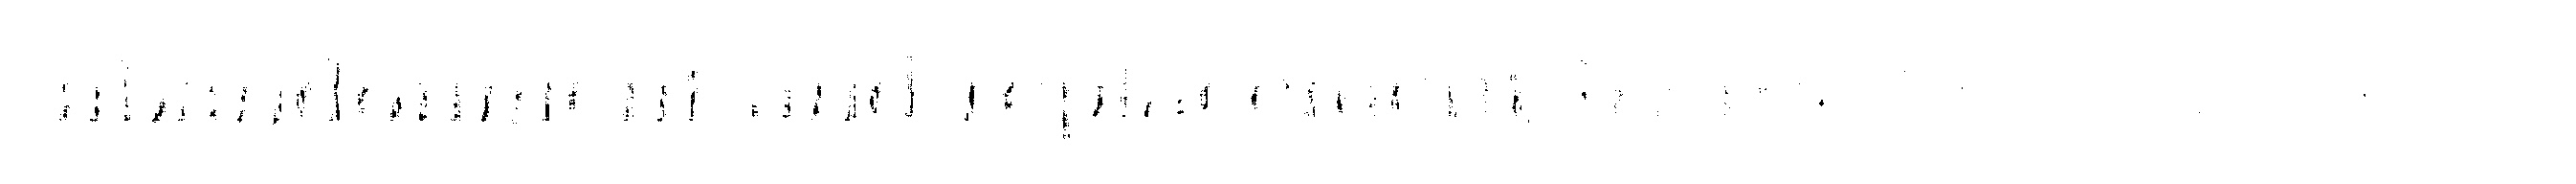
\includegraphics[width=1\textwidth]{obrazky/threshold_gauss(9,4).jpg}
     	Obrázek-1: Gaussovský adaptivní práh\\
     	
\includegraphics[width=1\textwidth]{obrazky/threshold_gauss(15,2).jpg}
     	Obrázek-2: Gaussovský adaptivní práh s jinými parametry\\
		
\includegraphics[width=1\textwidth]{obrazky/threshold_mean(9,4).jpg}
     	Obrázek-3: Adaptivní práh\\
     	
\includegraphics[width=1\textwidth]{obrazky/threshold_otsu.jpg}
     	Obrázek-4: Otsuovo práh\\
     	\end{center}
\end{frame}
\begin{frame}
\frametitle{Další úpravy}
\begin{itemize}
\item Grayscale - převede obrázek do úrovní šedi
\item Rozmazání - nějakým způsobem průměruje okolí pixelu
\item Škálování - změna velikosti obrázku
\item Odstranění šumu
\end{itemize}
\end{frame}

\subsection{B-MOD}
\begin{frame}
\frametitle{B-MOD}
		\begin{columns}
		\begin{column}{0.5\textwidth}
\begin{itemize}
\item \emph{Brno Mobile OCR Dataset} - z VUTBR
\item Rozmanitý: foceno různými zařízením za různých světelných vzdáleností z různých úhlů
\item Rozstřihané fotky po jednotlivých řádcích
\end{itemize}
		\end{column}
		\begin{column}{0.5\textwidth}
    	\begin{center}
     	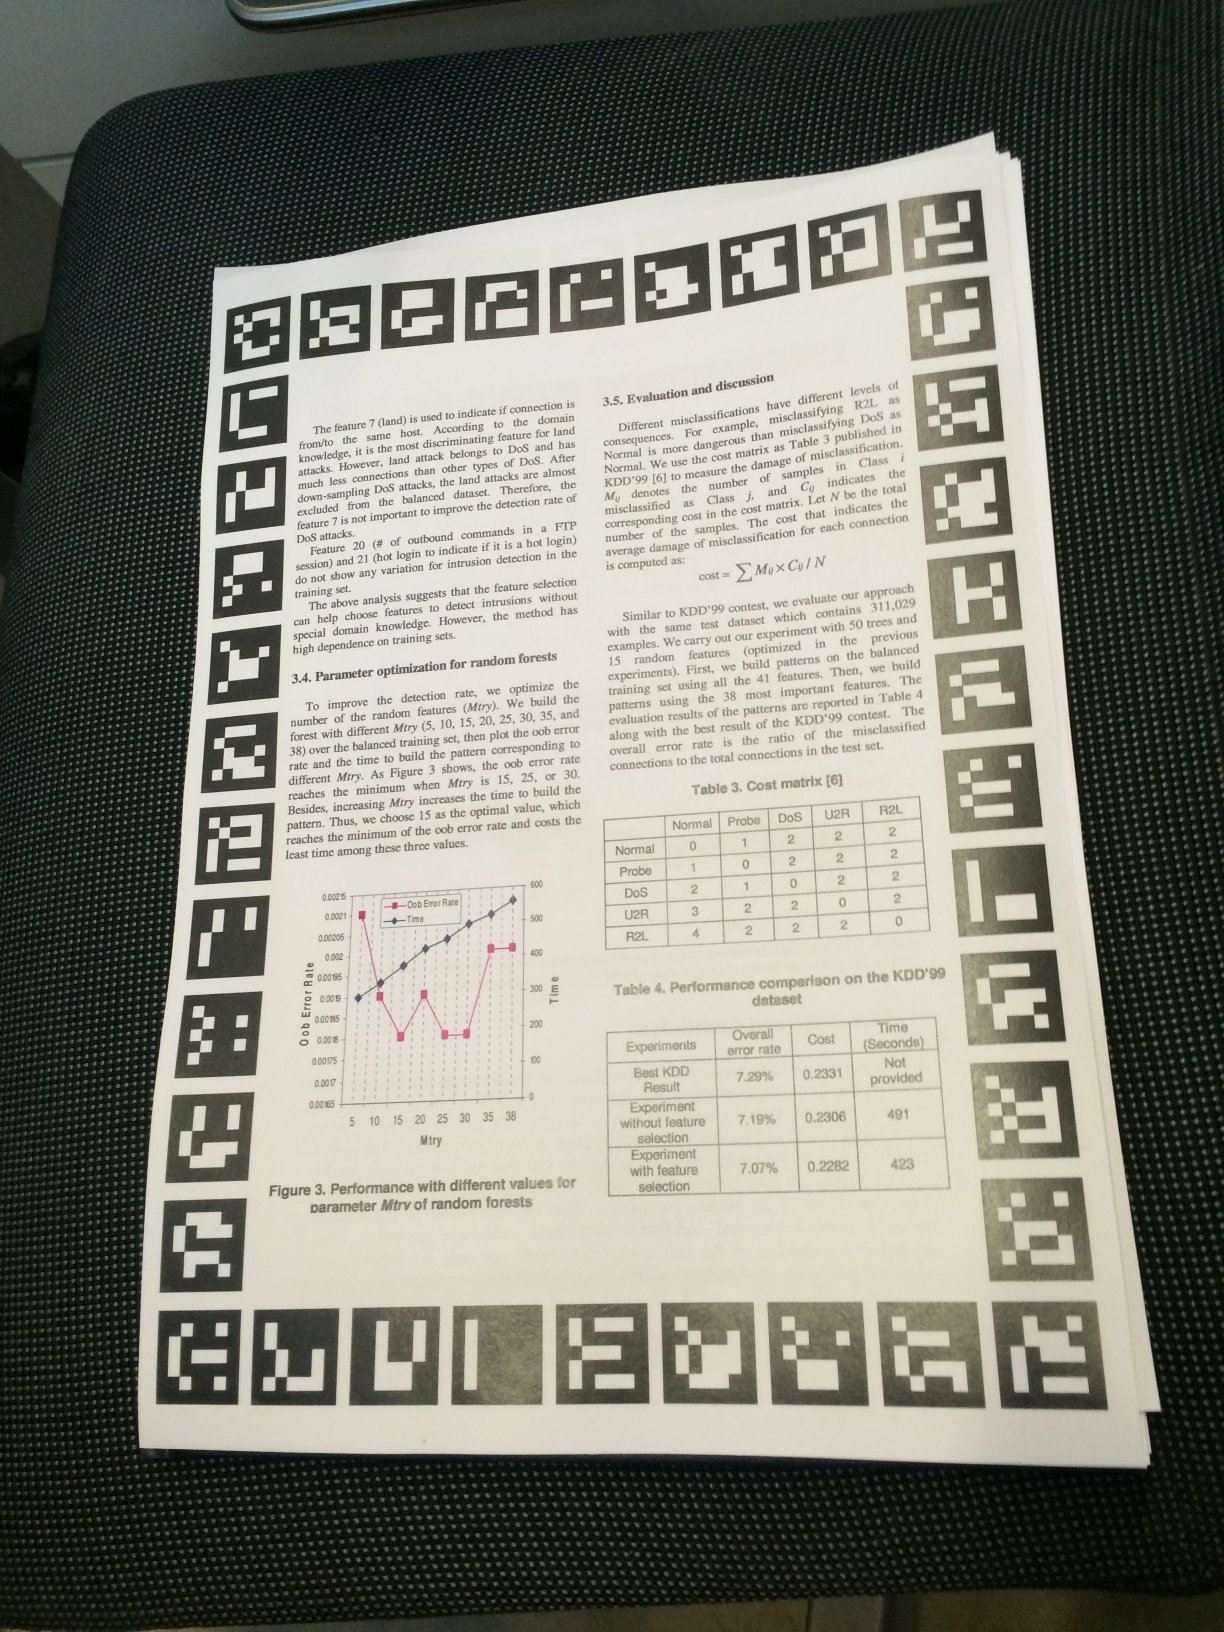
\includegraphics[width=0.5\textwidth]{img/bmod-sample.jpg}\\
     	Obrázek-5: Ukázka z datasetu
     	\end{center}
		\end{column}
		\end{columns}
\end{frame}
\begin{frame}
\frametitle{Mnou použité}
    	\begin{center}
     	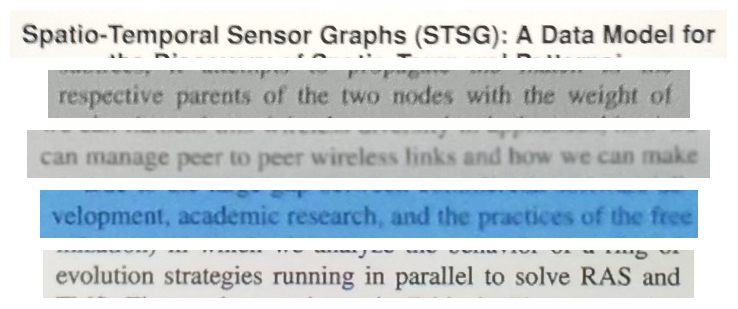
\includegraphics[width=1\textwidth]{img/bmod-easy.png}\\
     	Obrázek-6: Po řádcích
     	\end{center}
\end{frame}
\begin{frame}
\frametitle{Mnou použité 2}
		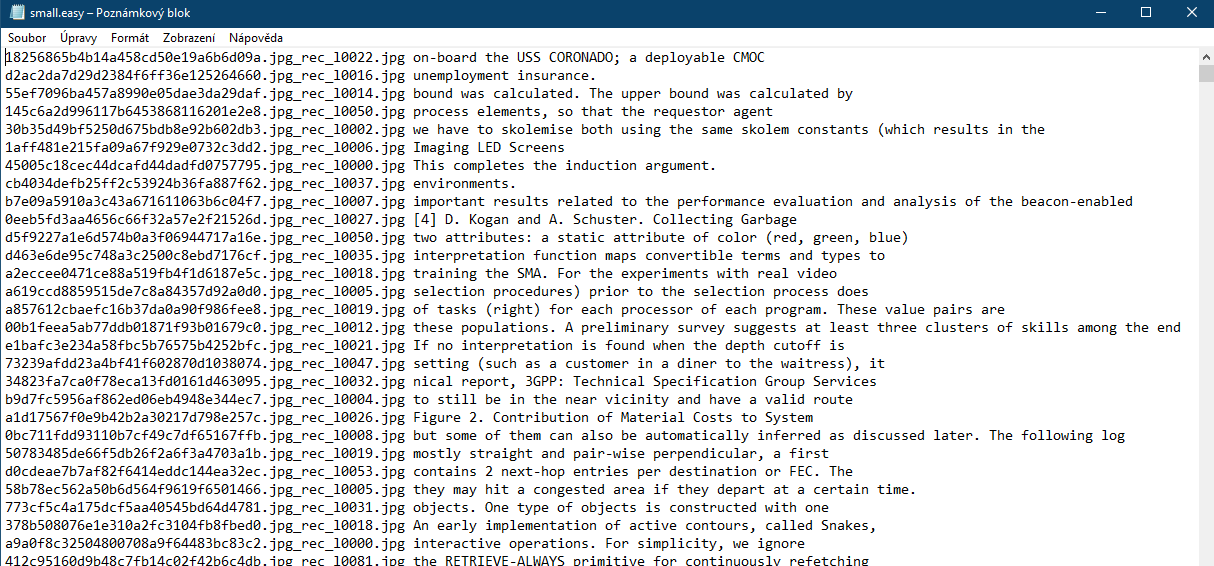
\includegraphics[width=1\textwidth]{img/b-mod-text.png}\\
     	Obrázek-7: Textový soubor se správným řešením
\end{frame}
\section{Postup}
\begin{frame}
\frametitle{Cíle a automatizace}
\begin{itemize}
\item Zjistit, jak upravit obrázek, tak aby se zlepšili výsledky Tesseractu
\item Zkusit velké množství úprav obrázků, zkusit rozpoznat Tesseractem a porovnat úspěšnosti
\end{itemize}
\end{frame}
\subsection{Praxe: OpenCV}
\begin{frame}
\frametitle{OpenCV}
\begin{itemize}
\item Vytvořil jsem si kódy jednotlivým funkcím
\item Program, který je vykoná v takovém pořadí v jakém jsou předloženy
\item Potřebné informace získá program z jedné řádky v textovém dokumentu
\item Program provede operaci pro všechny řádky v souboru
\end{itemize}
\end{frame}
\begin{frame}
\frametitle{OpenCV parametry}
\centering
		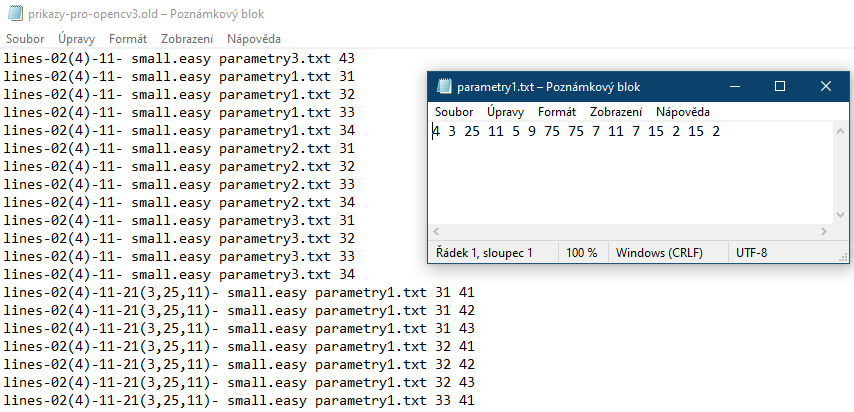
\includegraphics[width=1.1\textwidth]{img/pro-OpenCV.png}\\
     	Obrázek-8: Textový soubor pro OpenCV
\end{frame}
\subsection{Praxe: Tesseract}
\begin{frame}
\frametitle{Tesseract a pytesseract}
\begin{itemize}
\item Je nutné dobře nainstalovat Tesseract
\item Je třeba ho nastavit jako příkaz v cmd
\item A propojit s Pythonem pomocí \emph{pytesseractu}
\item Poté zavolat Tesseract a uložit jeho výstup do textového souboru
\end{itemize}
\end{frame}
\begin{frame}
\frametitle{Příkazy pro Tesseract}
\centering
	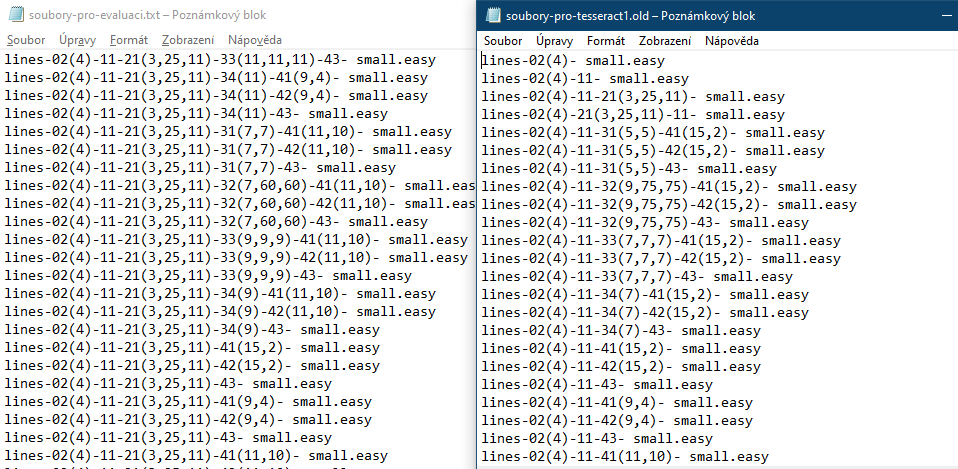
\includegraphics[width=1.15\textwidth]{img/pro-tesseract-evaluaci.png}\\
	Obrázek-9: Textový soubor pro Tesseract
\end{frame}
\subsection{Praxe: Měření úspěšnosti}
\begin{frame}
\frametitle{Výstup Tesseractu}
\centering	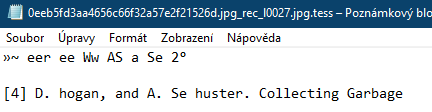
\includegraphics[width=1.1\textwidth]{img/vystup-tess.png}\\
Obrázek-10: Textový soubor vytvořený Tesseractem
\end{frame}
\begin{frame}
\frametitle{Úspěšnost}
\begin{itemize}
\item Převede znak nové řádky na mezeru
\item Rozdělí podle mezer
\item Ve vzniklém poli hledá slova v řešení (to také rozdělíme podle mezer)
\item Vypočítá jaké procento slov to nenašlo, tj. byly chybně identifikovány
\end{itemize}
\end{frame}
\section{Závěr}
\subsection{Výsledky}
\begin{frame}
\frametitle{Výstup programu}
\centering
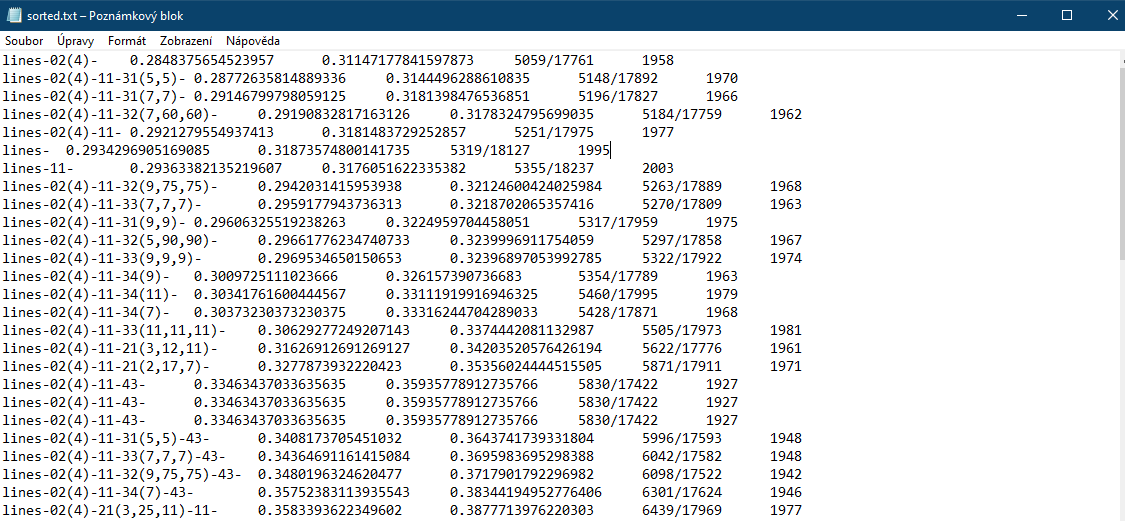
\includegraphics[width=1.1\textwidth]{img/vysledky.png}\\
Obrázek-11: Textový soubor vytvořený evaluačním programem
\end{frame}
\begin{frame}
\frametitle{Tabulka}
\centering
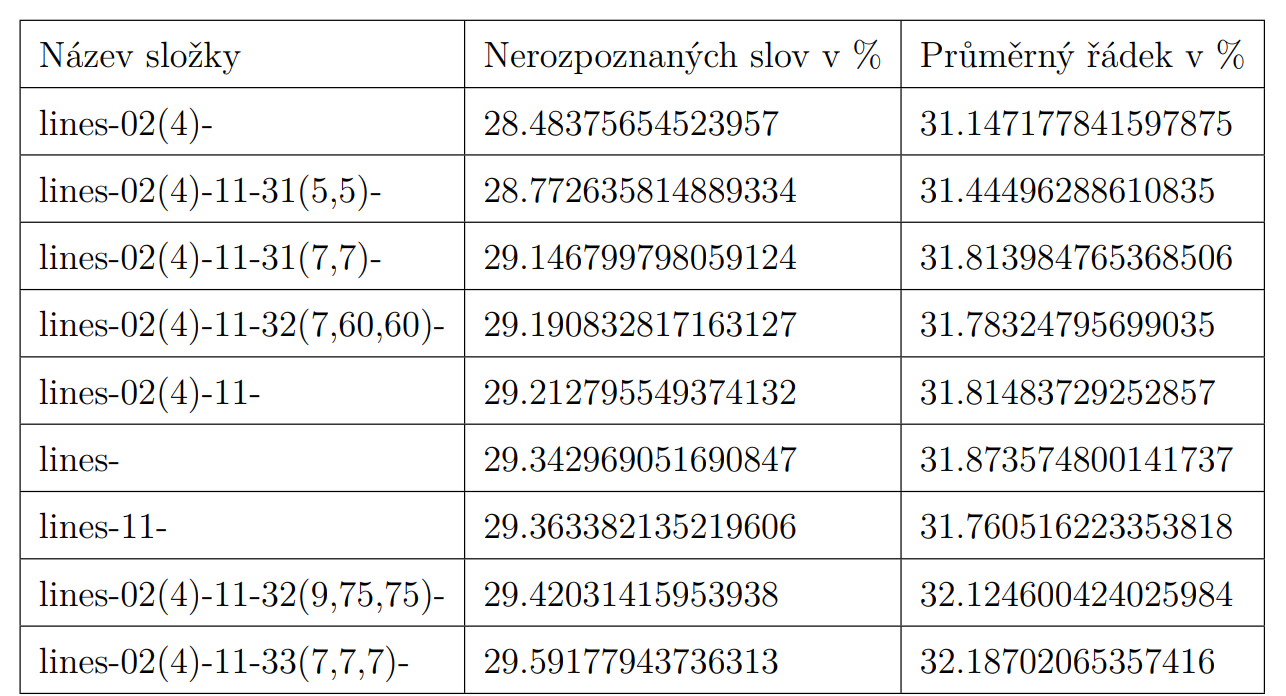
\includegraphics[width=1\textwidth]{img/vysledky-tabulka.png}\\
Obrázek-12: Tabulka nejlepších kombinací
\end{frame}
\begin{frame}
\frametitle{Tabulka}
\centering
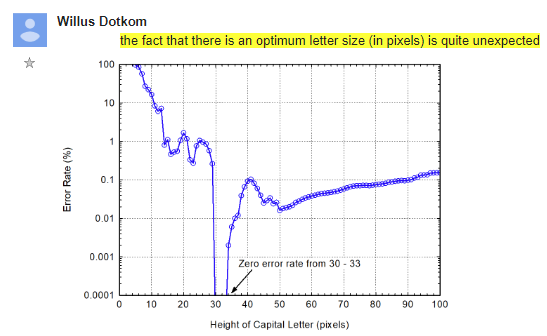
\includegraphics[width=1\textwidth]{img/dotkom.png}\\
Obrázek-13: Optimální velikost pro Tesseract 
\end{frame}
\subsection{Zhodnocení}
\begin{frame}
\frametitle{Nedostatky}
\begin{itemize}
\item Nepřehledné kódování funkcí OpenCV
\item Nesystematické procházení možností 
\end{itemize}
\end{frame}
\subsection{Konec}
\begin{frame}
\frametitle{Děkuji za pozornost!}
\framesubtitle{Pokud máte zájem, položte dotazy!}
\centering
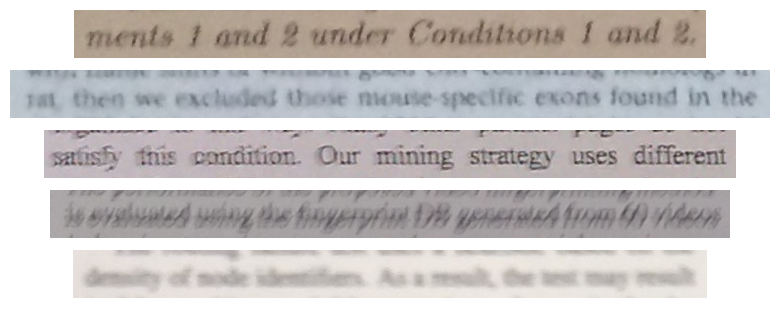
\includegraphics[width=1\textwidth]{img/bmod-medium.png}\\
%Obrázek-14: Ukázka z B-MOD 
\end{frame}
\end{document}